\documentclass[12pt,a4paper,titlepage,spanish]{article} 
\usepackage{babel}
\usepackage [T1]{fontenc}
\usepackage [latin1]{inputenc}
\usepackage{graphicx}
\usepackage{amssymb}
\usepackage{amsmath}
\usepackage{setspace}
\usepackage{epsfig}
\usepackage{enumerate}
\usepackage{float}
\usepackage{array}
\usepackage{cancel}
%\usepackage{arcs}
\usepackage[usenames,dvipsnames]{color}

	  \oddsidemargin 0in
      \textwidth 6.75in
      \topmargin 0in
      \textheight 10.0in
      \parindent 0em
      \parskip 2ex
\usepackage{anysize}
\marginsize{3cm}{2cm}{1.0cm}{1.0cm}
\pagestyle{plain}
\title{
\begin{Large}
 \begin{center}
		\underline{Informe simulaciones TP03 - GNA Von NewMann}\\
		\underline{Curso: } 6to 1ra\\
		\underline{Turno: } Noche\\
		\underline{CPU: } Intel Core 2 Duo E6600\\
      \end{center}
\end{Large}
}
\author{Vileri�o, Silvio}

\begin{document}
\maketitle
\setcounter{page}{2}
\tableofcontents
\newpage

\subsection{Introducci�n}
Esta simulaci�n se desarrolla con el fin de comprobar la calidad del generador de numeros aleatorios (GNA) desarrollado por John, Von NewMann, conocido como el m�todo de los cuadrados centrados.
Se realizaran 2 algoritmos, uno basado en Cadenas de caracteres, y otro puramente num�rico.\\
Se le realizan las siguientes pruebas:\\
\begin{itemize}
	\item Se calcula un promedio $ \bar X $ de 1000000 n�meros generados al azar.\\
		$ \bar X = \frac{\displaystyle{\sum_{k=1}^n} {a_k}}{n}, n=1000000 $
	\item Se calcula la dispersi�n $ \sigma^2 $ entre cada n�mero generado y el promedio obtenido anteriormente.\\
		$ \sigma^2 = \frac{\displaystyle{\sum_{i=1}^n {(X_i - \bar X)^2}}}{n}, n=1000000, \bar X \longrightarrow $ promedio
	\item Se confecciona un histograma donde se registran la cantidad de n�meros generados entre 0,0 exclusive y 0,1 exclusive, en 10 intervalos de 0,1
	\item Se calcula $ \bar f $, la frecuencia promedio de los intervalos.\\
	$ \bar f=\frac{\displaystyle{\sum_{i=1}^n {k_i}}}{n},n=10, k_i \longrightarrow $ frecuencia registrada en cada intervalo.
	\item Se calcula la dispersion $ \sigma^2_{hist} $ entre las frecuencias del histograma y la frecuencia promedio obtenida anteriormente\\
	 $ \sigma^2_{hist}=\frac{\displaystyle{\sum_{i=1}^n {(F_i - \bar f)^2}}}{n}, n=10 $
	 \item Se realizan dos pruebas gr�ficas en las que se generan 250000 puntos al azar en un �rea de $ 500 \times 500 $ p�xeles. \begin{itemize}
	 											\item Paralelo: se toman dos GNA con distinta semilla , para x e y .
	 											\item Serie: se toman dos GNA y se mantiene esta relaci�n para la generaci�n de valores de x e y :$ x=GNA(GNA(x)) $, previamente x siendo la semilla inicial.
	 												 											
	 										\end{itemize}
\end{itemize}
\newpage
\subsection{Resultados GNA Cadena de Caracteres}
Luego de realizar la simulaci�n, se obtuvieron los siguientes resultados: \\

\begin{itemize}
\item Promedio $ \longrightarrow  \bar X = 0.46910603604175966 $ 
 \item Dispersi�n $ \longrightarrow \sigma^2 = 0.08150241710671692 $ 
	\item Histograma: \begin{itemize}	
			\item Intervalo $ \left( 0.0 ; 0.1 \right)= 72730 $
			\item Intervalo $ \left[ 0.1 ; 0.2 \right)= 163633 $
			\item Intervalo $ \left[ 0.2 ; 0.3 \right)= 145450 $
			\item Intervalo $ \left[ 0.3 ; 0.4 \right)= 90910 $
			\item Intervalo $ \left[ 0.4 ; 0.5 \right)= 145449 $
			\item Intervalo $ \left[ 0.5 ; 0.6 \right)= 54549 $
			\item Intervalo $ \left[ 0.6 ; 0.7 \right)= 18184 $
			\item Intervalo $ \left[ 0.7 ; 0.8 \right)= 90911 $
			\item Intervalo $ \left[ 0.8 ; 0.9 \right)= 145456 $
			\item Intervalo $ \left[ 0.9 ; 1.0 \right)= 72728 $
		\end{itemize}
		\item Frecuencia Promedio $ \longrightarrow \bar f = 100000 $
		\item Dispersi�n del Histograma $ \longrightarrow \sigma^2_{freq. hist.} = 2.0659024888 \times 10^{9} $
\end{itemize}
\newpage

\subsection{Resultados GNA Num�rico}
Luego de realizar la simulaci�n, se obtuvieron los siguientes resultados: \\

\begin{itemize}
\item Promedio $ \longrightarrow  \bar X = 0.5326296892822701 $ 
 \item Dispersi�n $ \longrightarrow \sigma^2 = 0.09269363308858188 $ 
	\item Histograma: \begin{itemize}	
\item Intervalo $ \left( 0.0 ; 0.1 \right)= 126725 $
\item Intervalo $ \left[ 0.1 ; 0.2 \right)= 56370 $
\item Intervalo $ \left[ 0.2 ; 0.3 \right)= 70442 $
\item Intervalo $ \left[ 0.3 ; 0.4 \right)= 112656 $
\item Intervalo $ \left[ 0.4 ; 0.5 \right)= 84528 $
\item Intervalo $ \left[ 0.5 ; 0.6 \right)= 56373 $
\item Intervalo $ \left[ 0.6 ; 0.7 \right)= 140824 $
\item Intervalo $ \left[ 0.7 ; 0.8 \right)= 98605 $
\item Intervalo $ \left[ 0.8 ; 0.9 \right)= 112684 $
\item Intervalo $ \left[ 0.9 ; 1.0 \right)= 140793 $
		\end{itemize}
\item Frecuencia Promedio $ \longrightarrow \bar f = 100000 $
\item Dispersi�n del Histograma $ \longrightarrow \sigma^2_{freq. hist.} = 9.287847844 \times 10^{8} $
\end{itemize}
\newpage

\subsection{Im�genes Cadenas de caracteres}
\underline{Histograma}\\
\begin{center}
	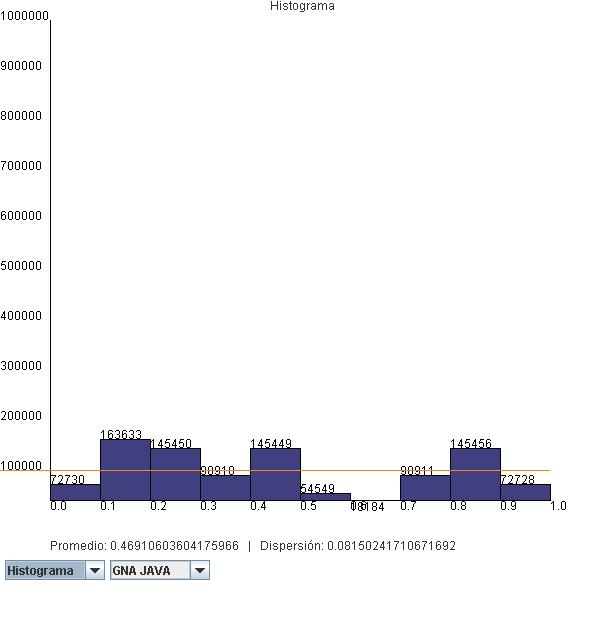
\includegraphics[scale=0.75]{String/Histograma.jpg}
\end{center}
\newpage
\underline{Test Gr�fico Paralelo}
\begin{center}
	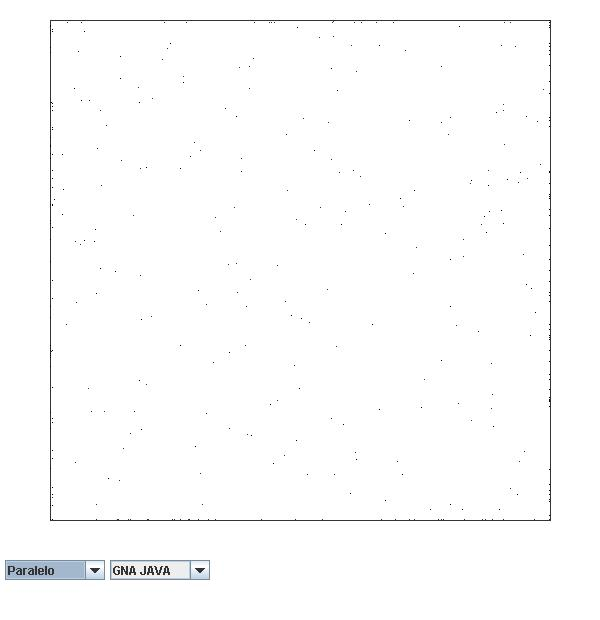
\includegraphics[scale=0.75]{String/Paralelo.jpg}
\end{center}
\newpage
\underline{Test Gr�fico Serie}
\begin{center}
	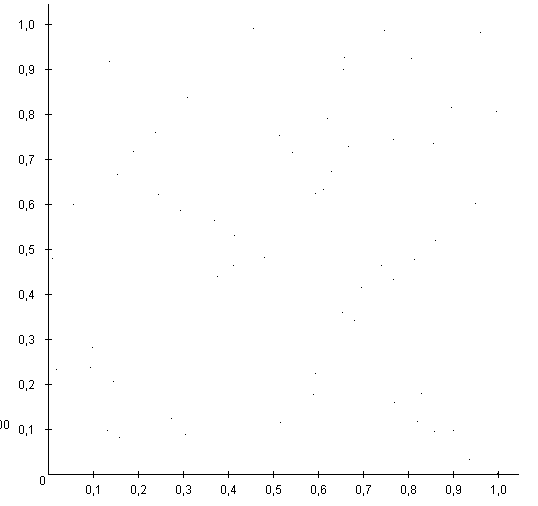
\includegraphics[scale=0.75]{String/Serie.jpg}
\end{center}
\newpage
\subsection{Im�genes Num�rico}
\underline{Histograma}\\
\begin{center}
	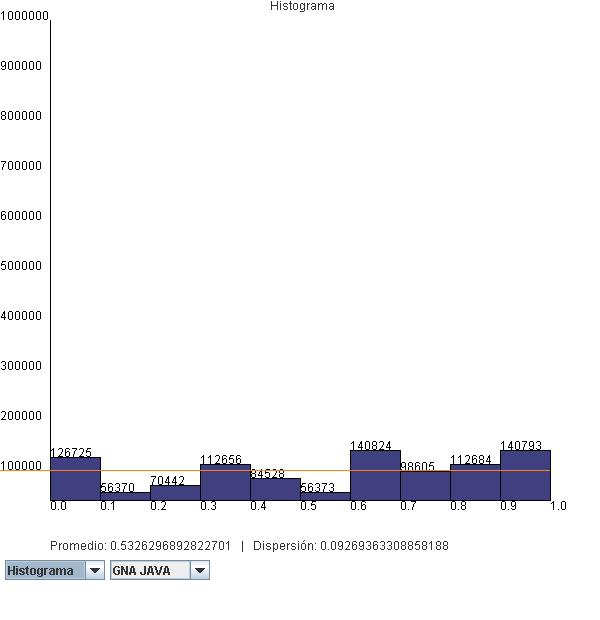
\includegraphics[scale=0.75]{Numeric/Histograma.jpg}
\end{center}
\newpage
\underline{Test Gr�fico Paralelo}
\begin{center}
	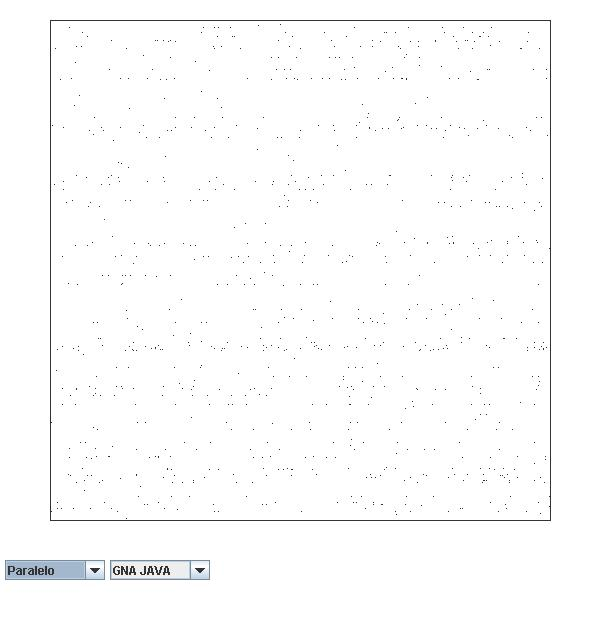
\includegraphics[scale=0.75]{Numeric/Paralelo.jpg}
\end{center}
\newpage
\underline{Test Gr�fico Serie}
\begin{center}
	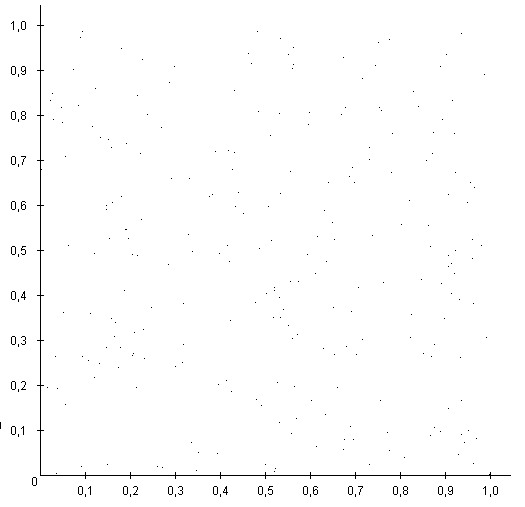
\includegraphics[scale=0.75]{Numeric/Serie.jpg}
\end{center}
\newpage
\subsection{Conclusi�n}
%Escribir conclusi�n.
\end{document}